\documentclass[12pt]{article}
\usepackage{amsfonts}
\usepackage{amsthm}
\usepackage{amsmath}
\usepackage[mathscr]{euscript}
\usepackage{array}
\usepackage[thinlines]{easytable}
\usepackage{tikz}
\usepackage{pgfplots}
\usepackage[margin=2cm]{geometry}
\usepackage{graphicx}
\usepackage{xcolor}
\usepackage[utf8]{inputenc}
\usepackage[T1]{fontenc}
\usepackage[portuguese]{babel}
\usepackage[backend=biber, style=numeric]{biblatex} %Imports biblatex package
\addbibresource{references.bib} %Import the bibliography file

\usepackage{lipsum} % Pode tirar esse :D
\usepackage{listings}
\usepackage{color}

\definecolor{dkgreen}{rgb}{0,0.6,0}
\definecolor{gray}{rgb}{0.5,0.5,0.5}
\definecolor{mauve}{rgb}{0.58,0,0.82}

\lstset{frame=tb,
	language=C++,
	aboveskip=3mm,
	belowskip=3mm,
	showstringspaces=false,
	columns=flexible,
	basicstyle={\small\ttfamily},
	numbers=none,
	numberstyle=\tiny\color{gray},
	keywordstyle=\color{blue},
	commentstyle=\color{dkgreen},
	stringstyle=\color{mauve},
	breaklines=true,
	breakatwhitespace=true,
 	tabsize=3
}

\def\be{\begin{equation}}
	\def\ee{\end{equation}}
\def\bee{\begin{equation*}}
	\def\eee{\end{equation*}}
\def\bea{\begin{eqnarray*}}
	\def\eea{\end{eqnarray*}}
\def\beaa{\begin{eqnarray}}
	\def\eeaa{\end{eqnarray}}

\def\bl{\begin{lemma}}
	\def\el{\end{lemma}}
\def\bt{\begin{theorem}}
	\def\et{\end{theorem}}
\def\bc{\begin{corollary}}
	\def\ec{\end{corollary}}

\def\bp{\begin{proof}}
	\def\ep{\end{proof}}

\def\bd{\begin{definition}}
	\def\ed{\end{definition}}
\def\br{\begin{remark}}
	\def\er{\end{remark}}

\def\bex{\begin{exercise}}
	\def\eex{\end{exercise}}
\def\bexa{\begin{example}}
	\def\eexa{\end{example}}
\def\bm{\begin{method}}
	\def\em{\end{method}}

\def\benu{\begin{enumerate}}
	\def\eenu{\end{enumerate}}
\def\bpr{\begin{proposition}}
	\def\epr{\end{proposition}}

\def\f{\frac}
\def\del{\partial}


\def\R{\mathbb{R}}
\def\K{\mathbb{K}}
\def\C{\mathbb{C}}
\def\I{\mathbb{I}}
\def\Z{\mathbb{Z}}
\def\Q{\mathbb{Q}}
\def\N{\mathbb{N}}

\def\cd{\cdot}

\def\v#1{{\boldsymbol{#1}}}
\def\ve#1{\hat{\boldsymbol#1}}

\def\l{\left}
\def\r{\right}
\def\la{\l\langle}
\def\ra{\r\rangle}
\def\div{\nabla\cdot}
\def\curl{\nabla\times}
\def\grad{\nabla}
\def\lap{\nabla^2}
\def\e{\varepsilon}

\def\s{\quad}
\def\ss{\qquad}
\def\infi{\infty}
\def\p{\partial}
\def\u{\cup}%union of two sets
\def\i{\cap}%intersection of two sets
\def\ds{\oplus}

\newtheorem{theorem}{Theorem}[section]
\newtheorem{corollary}{Corollary}[theorem]
\newtheorem{lemma}[theorem]{Lemma}
\theoremstyle{definition}
\newtheorem{definition}{Definition}[section]
\newtheorem*{remark}{Remark}
\newtheorem{method}{Method}[section]
\newtheorem{example}{Example}[section]
\newtheorem{proposition}{Proposition}[section]



\newcommand\norm[1]{\left\lVert#1\right\rVert}

\DeclareMathOperator{\atan}{atan}
\DeclareMathOperator{\sech}{sech}
\DeclareMathOperator{\csch}{csch}
\DeclareMathOperator{\asinh}{asinh}
\DeclareMathOperator{\atanh}{atanh}
\DeclareMathOperator{\acoth}{acoth}
\DeclareMathOperator{\acosh}{acosh}
\DeclareMathOperator{\acsch}{acsch}
\DeclareMathOperator{\asech}{asech}
\DeclareMathOperator{\im}{Im}
\DeclareMathOperator{\D}{D}
\DeclareMathOperator{\Tr}{tr}
\DeclareMathOperator{\graph}{graph}
\DeclareMathOperator{\spann}{span}
\DeclareMathOperator{\aut}{Aut}
\DeclareMathOperator{\LAM}{LAM}
%\DeclareMathOperator{\det}{det}
%\DeclareMathOperator{\dim}{dim}

\title{Quantificação de Análise de Recorrência Eficiente na GPU}
\author{Lucas Froguel\\ Programação Paralela em GPUs}
\date{}

\begin{document}
	\maketitle
	
	\section{Introdução}
	
	Nesse trabalho foi feita uma implementação em paralelo na GPU do algoritmo descrito no artigo enviado ao professor. A ideia básica do algoritmo lá descrito é calcular a laminariedade usando pequenos blocos da matriz total chamados de microestados. Dentro de cada microestado, montamos um diagrama das linhas horizontais e calculamos a laminaridade por:
	\be\label{eq1}
		\LAM = \f{\sum_{v=v_\text{min}}^K vP(v)}{\sum_{v=1}^K vP(v)}
	\ee
	
	Assim, a ideia da implementação em GPU é fazer com que cada bloco processe um microestado, de modo que possamos ter o processamento simultâneo de vários microestados. O funcionamento do código está explicado nos comentários, mas aqui segue um resumo do código do kernel. 
	\begin{enumerate}
		\item Definir e alocar espaços
		\begin{lstlisting}
			__shared__ float mapx[Q], mapy[Q];
			__shared__ bool microstate[Q * Q];
			__shared__ int histogram[Q];
			int tid = threadIdx.x;
			int gtid = blockDim.x * blockIdx.x + threadIdx.x;
			int i, j;
			
			// get two random indexes 
			i = xrand[blockIdx.x];
			j = yrand[blockIdx.x];
		\end{lstlisting}
		\item Carregar os dados a serem processados da memória global para a shared memory
		\begin{lstlisting}
		// load data [i, i+Q] and [j, j+Q] to shared memory
		// each thread loads [tid, tid+blockDim, ...] until all elements are loaded
		for (int k = tid; k < Q; k = k + blockDim.x){
			// i, j are such that i + Q, j + Q < N
			mapx[k] = d_map[i + k];
			mapy[k] = d_map[j + k];
			// clean histogram on shared memory
			histogram[k] = 0;
		}
		\end{lstlisting}
		\item Calcular o microestado
		\begin{lstlisting}
			// calculate CRP / microstate
			for (int k = tid; k < Q * Q; k = k + blockDim.x){
				bool m = 0;
				int iq = k % Q, jq = k / Q;
				float val = abs(mapx[iq] - mapy[jq]);
				if (val < e) m = 1;
				microstate[k] = m;
			}
		\end{lstlisting}
		\item Montar o histograma
		\begin{lstlisting}
			// each thread will look for lines in one row of the microstate
			// values will be CRP[tid, k], k\in[0, Q-1]
			// assumes Q < threadsPerBlock (which is very reasonable, given the amount of shared memory per block)
			if (tid < Q){
				int line_length = 0;
				for (int k = 0; k < Q; k++){
					if (microstate[k + tid * Q] == 1){
						line_length += 1;
						if (k == Q - 1){
							atomicAdd(&histogram[line_length-1], 1);
							line_length = 0;
						}
					}
					else if (line_length > 0 && microstate[k + tid * Q] == 0){
						atomicAdd(&histogram[line_length-1], 1);
						line_length = 0;
					} 
				}
			}
		\end{lstlisting}
		\item Fazer a soma da Eq.(\ref{eq1})
		\begin{lstlisting}
			// should be a cheap/fast operation, but has to be done on one thread
			if (tid == 0){
				float LAM = 0, total = 0;
				for (int k = 0; k < Q; k++){
					if (k + 1 >= lmin){
						LAM += histogram[k] * (k+1);
					}
					total += histogram[k] * (k+1);
				}
				if (total != 0) d_LAM[blockIdx.x] = LAM / total;
			}
		\end{lstlisting}
	\end{enumerate}

	Para a CPU tudo que resta é gerar números aleatórios, carregar e transferir dados para a GPU e iniciar o kernel. 

	\section{Resultados}
	
	Para avaliar a eficiência, os resultados da GPU foram comparados com duas implementações no mesmo algoritmo na cpu (uma usando apenas 1 thread e outra usando a versão paralela), ambas em julia, e também com o PyRQA, que é uma implementação paralela na GPU do algoritmo tradicional (e usa OpenCL). 
	
	A máquina utilizada possuí um i7-10700KF (com 16 threads) e uma RTX3060. As informações detalhadas de ambas estão no repositório na pasta PC-data. 
	
	Os resultados estão mostrados na Fig.(\ref{fig:times}) e na Tab.(\ref{tab1}). O maior speedup, curiosamente, foi com $ind=6$ contra o PyRQA e foi de $\sim 3,2\times10^5$ vezes. Contra a cpu, foi em $ind=10$ e foi de cerca de $\sim 2000$ vezes. Isso demonstra que a implementação em GPU da nova abordagem é extremamente mais rápida que a implementação em GPU existente e do que as de CPU. Apesar de ambos os resultados serem esperados, pois esse algoritmo é, de fato, mais rápido e a GPU é realmente mais rápida do que a CPU. 
	
	\begin{figure}
		\centering
		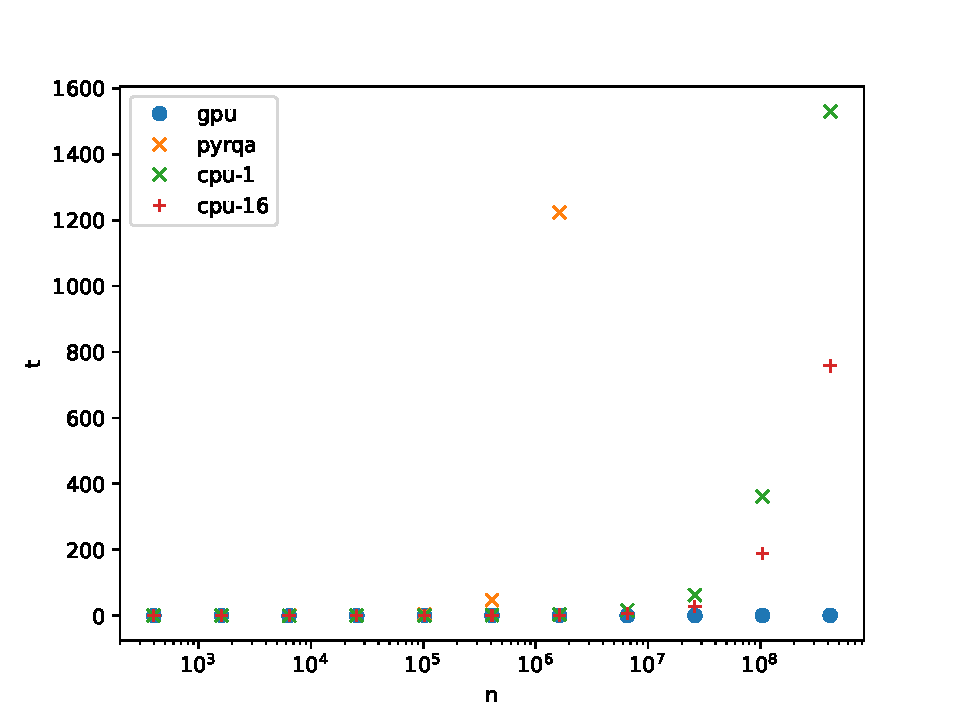
\includegraphics[width=0.7\linewidth]{times}
		\caption{Figura com os tempos de cálculo das 4 implementações consideradas}
		\label{fig:times}
	\end{figure}
	
	\begin{table}[]
		\begin{tabular}{|c|c|c|c|c|c|c|}
			\hline
			ind & n         & time\_gpu & time\_cpu   & time\_cpu\_multi & time\_pyrqa & gpu\_min\_speedup \\ \hline
			0   & 400       & 0.000044  & 0.000961    & 0.049372         & 0.084893    & 21.8              \\ \hline
			1   & 1600      & 0.000034  & 0.003351    & 0.001733         & 0.057727    & 51.0              \\ \hline
			2   & 6400      & 0.000039  & 0.023179    & 0.004588         & 0.085305    & 117.6             \\ \hline
			3   & 25600     & 0.000086  & 0.067011    & 0.024826         & 0.320447    & 288.7             \\ \hline
			4   & 102400    & 0.000265  & 0.231871    & 0.123956         & 3.011581    & 468.0             \\ \hline
			5   & 409600    & 0.000967  & 0.920062    & 0.393596         & 47.047580   & 407.4             \\ \hline
			6   & 1638400   & 0.003784  & 3.969902    & 1.489342         & 1222.607544 & 393.9             \\ \hline
			7   & 6553600   & 0.014997  & 16.227974   & 5.941865         & NaN         & 396.15            \\ \hline
			8   & 26214400  & 0.060014  & 61.813792   & 27.755246        & NaN         & 462.6             \\ \hline
			9   & 104857600 & 0.241047  & 360.439228  & 188.912355       & NaN         & 783.9             \\ \hline
			10  & 419430400 & 0.879212  & 1529.509376 & 757.977858       & NaN         & 862.3             \\ \hline
		\end{tabular}
		\caption{Essa tabela mostra os valores de tempo para o calculo da LAM para cada implementação e o speedup mínimo da gpu.}
		\label{tab1}
	\end{table}

\end{document}
